\subsection{Mathematical modelling}

\noindent To determine the static performance characteristics of the
aircraft as well as solve the minimum time problems set we need sufficient
mathematical models to work with. For this part \textit{the aircraft is
modelled as a point mass system}. With this simplification in mind the forces
acting on the airplane are given in fig.~\ref{fig:forces_sketch}.

\begin{figure}[H]
    \centering
    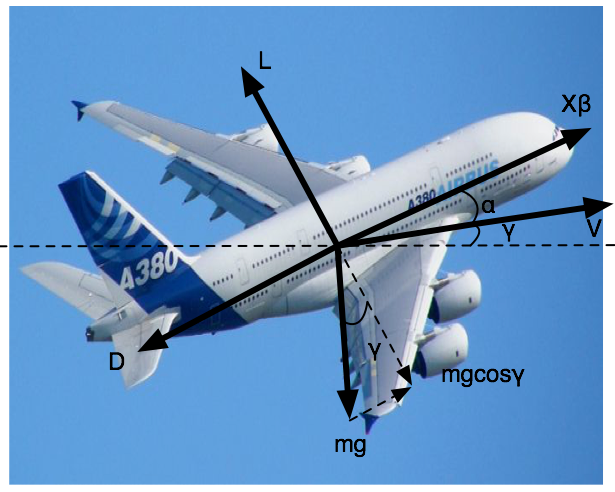
\includegraphics[width=0.8\textwidth]{forces_sketch}
    \caption{Forces acting on the point mass system}
    \label{fig:forces_sketch}
\end{figure}

\noindent The set of differential equations governing the motion of the aircraft is stated 
below (Eq. \ref{eqn:pointmass1}-\ref{eqn:pointmass5}):

\begin{align}
    m\dot{V}&= Tcos(\alpha + \epsilon) - D - mgsin\gamma  \label{eqn:pointmass1}\\
    mV\dot{\gamma}&= Tsin(\alpha + \epsilon) + L - mgcos\gamma \label{eqn:pointmass2}\\
    \dot{h} &= Vsin\gamma \label{eqn:pointmass3}\\
    \dot{x}_{\epsilon} &= Vcos\gamma \label{eqn:pointmass4}\\
    \dot{m} &= -b \label{eqn:pointmass5}
\end{align}

\nomenclature{$V$}{Total Aircraft Velocity}%
\nomenclature{$m$}{Aircraft total mass}%
\nomenclature{$h$}{Aircraft altitude}%
\nomenclature{$L$}{Lift force}%
\nomenclature{$D$}{Drag force}%
\nomenclature{$x_{\epsilon}$}{Aircraft horizontal position displacement}%
\nomenclature{$\gamma$}{Fligth Path angle}%
\nomenclature{$\alpha$}{Angle of attack}%
\nomenclature{$\epsilon$}{Thrust angle}%
\nomenclature{$\theta$}{Angle of attitude}%


\noindent To simplify the numerical solving procedure, \textit{we neglect the evolution of 
the horizontal displacement} (Eq. ~\ref{eqn:pointmass4}) Instead, we calculate (in the end)
the total distance covered by the aircraft during the simulation by integrating through 
the velocity values computed:

\begin{equation}
    x_E(t) = \int_0^{t_f} \! V(t) cos\gamma(t) dt
    \label{eqn:integral_distance}
\end{equation}

\noindent To simplify the model even further we assume that the acceleration perpendicular to
the flight path is negligble ($\dot{\gamma} = 0$) so that the system evolution is defined only by eq.~\ref{eqn:pointmass1}
,\ref{eqn:pointmass3},\ref{eqn:pointmass5}:
\begin{align}
    m\dot{V}&= Tcos(\alpha + \epsilon) - D - mgsin\gamma  \notag\\
    \dot{h} &= Vsin\gamma \notag\\
    \dot{m} &= -b \notag
\end{align}
\begin{center}Final set of differential equations\end{center}



\subsubsection{Static performance - Methodology}

To derive the excess thrust and SEP-Graphs we first \textit{trim the aircraft} 
to obtain a flyable situation. This is done by solving eq.~\ref{eqn:pointmass2} 
for $\dot{\gamma} = 0$ and finding a valid-for-flight $\alpha$. Then for given 
mach number and altitude compute the aerodynamic coefficients, the thrust the drag
and the lift
\footnote{
The model for the lift force is the following:
\begin{equation}
    L = C_Lq_{dyn}S_{ref} \Rightarrow L = C_{La}(a_0 - c_{L0})q_{dyn}S_{ref}\notag
\end{equation}
where, one can observe that $C_L$ is not a non-dimensional quantity. That is due 
to the format of the aerodynamic data used for the simulation.
}

based on the given model, and finally we compute the excess thrust 
by computing the right-hand side of eq.~\ref{eqn:pointmass1}. Finally we use the following
equation for the computation of the Specific Excess Power.

\begin{equation}
    SEP = \frac{T_{EX}\,V}{mg}
    \label{eqn:SEP}
\end{equation}

\nomenclature{$T_{ex}$}{Excess thrust}%
\nomenclature{$SEP$}{Specific Excess Power}%

\subsubsection{Minimum time problems set - Methodology}
To find an optimum trajectory for the airplane to fly for different scenarios we
first find a `flyable' situation, as we mentioned previously, we find a valid $\alpha$
for the initial mach number and altitude and then we \textit{time integrate} the final set of 
differential equations derived, using $\gamma$ as input to the system. 
So the task at hand using this strategy is to find the ideal $\gamma$ input for 
achieving the defined goal each time.




